\documentclass[ignoreframetext]{beamer}
\usepackage[utf8]{inputenc}
\usepackage[T1]{fontenc}
\usepackage[swedish]{babel}
\usepackage{booktabs}

\usepackage[natbib,style=alphabetic,maxbibnames=99]{biblatex}
\addbibresource{slides.bib}

\usepackage[all]{foreign}
\renewcommand{\foreignfullfont}{}
\renewcommand{\foreignabbrfont}{}

\usepackage{newclude}
\usepackage{import}

\usepackage[strict]{csquotes}
\usepackage[single]{acro}

\usepackage{subcaption}

\usepackage[noend]{algpseudocode}
\usepackage{xparse}

\let\email\texttt

\usepackage[outputdir=ltxobj]{minted}
\setminted{autogobble,fontsize=\footnotesize}

\usepackage{pythontex}
\setpythontexoutputdir{.}
\setpythontexworkingdir{..}

\usepackage{amsmath}
\usepackage{amssymb}
\usepackage{mathtools}
\usepackage{amsthm}
\usepackage{thmtools}
\usepackage[unq]{unique}
\DeclareMathOperator{\powerset}{\mathcal{P}}

\usepackage[binary-units]{siunitx}

\usepackage[capitalize]{cleveref}

\usepackage{import}

\usetheme{Berlin}
\setbeamertemplate{footline}%{miniframes theme}
{%
  \begin{beamercolorbox}[colsep=1.5pt]{upper separation line foot}
  \end{beamercolorbox}
  \begin{beamercolorbox}[ht=2.5ex,dp=1.125ex,%
    leftskip=.3cm,rightskip=.3cm plus1fil]{author in head/foot}%
    \leavevmode{\usebeamerfont{author in head/foot}\insertshortauthor}%
    \hfill%
    {\usebeamerfont{institute in head/foot}\usebeamercolor[fg]{institute in head/foot}\insertshortinstitute}%
  \end{beamercolorbox}%
  \begin{beamercolorbox}[ht=2.5ex,dp=1.125ex,%
    leftskip=.3cm,rightskip=.3cm plus1fil]{title in head/foot}%
    {\usebeamerfont{title in head/foot}\insertshorttitle} \hfill     \insertframenumber%
  \end{beamercolorbox}%
  \begin{beamercolorbox}[colsep=1.5pt]{lower separation line foot}
  \end{beamercolorbox}
}
\setbeamercovered{transparent}
\setbeamertemplate{bibliography item}[text]

\AtBeginSection[]{%
  \begin{frame}<beamer>
    \tableofcontents[currentsection]
  \end{frame}
}

\ProvideDocumentEnvironment{assumption}{o}{%
  \IfValueTF{#1}{%
    \begin{block}{Assumption: #1}
  }{%
    \begin{block}{Assumption}
  }
}{%
  \end{block}
}

\ProvideDocumentEnvironment{protocol}{o}{%
  \IfValueTF{#1}{%
    \begin{block}{Protocol: #1}
  }{%
    \begin{block}{Protocol}
  }
}{%
  \end{block}
}

\ProvideDocumentEnvironment{remark}{o}{%
  \IfValueTF{#1}{%
    \begin{alertblock}{Note: #1}
  }{%
    \begin{alertblock}{Note}
  }
}{%
  \end{alertblock}
}

\ProvideDocumentEnvironment{idea}{o}{%
  \IfValueTF{#1}{%
    \begin{block}{Idea: #1}
  }{%
    \begin{block}{Idea}
  }
}{%
  \end{block}
}

\ProvideDocumentEnvironment{question}{o}{%
  \setbeamercolor{block body}{bg=orange!15,fg=black}
  \setbeamercolor{block title}{bg=orange,fg=white}
  \setbeamercolor{local structure}{fg=orange}
  \IfValueTF{#1}{%
    \begin{block}{Question: #1}
  }{%
    \begin{block}{Question}
  }
}{%
  \end{block}
}

\ProvideDocumentEnvironment{exercise}{o}{%
  \setbeamercolor{block body}{bg=yellow!10,fg=black}
  \setbeamercolor{block title}{bg=yellow,fg=black}
  \setbeamercolor{local structure}{fg=yellow}
  \IfValueTF{#1}{%
    \begin{block}{Exercise: #1}
  }{%
    \begin{block}{Exercise}
  }
}{%
  \end{block}
}


\begin{document}
\title{Mer formatering och felhantering}
\author{Daniel Bosk}
\institute{KTH EECS}

\maketitle

\mode<all>
\mode*

\section{Formattera strängar}

\subsection{Dokumentation}

\begin{frame}
  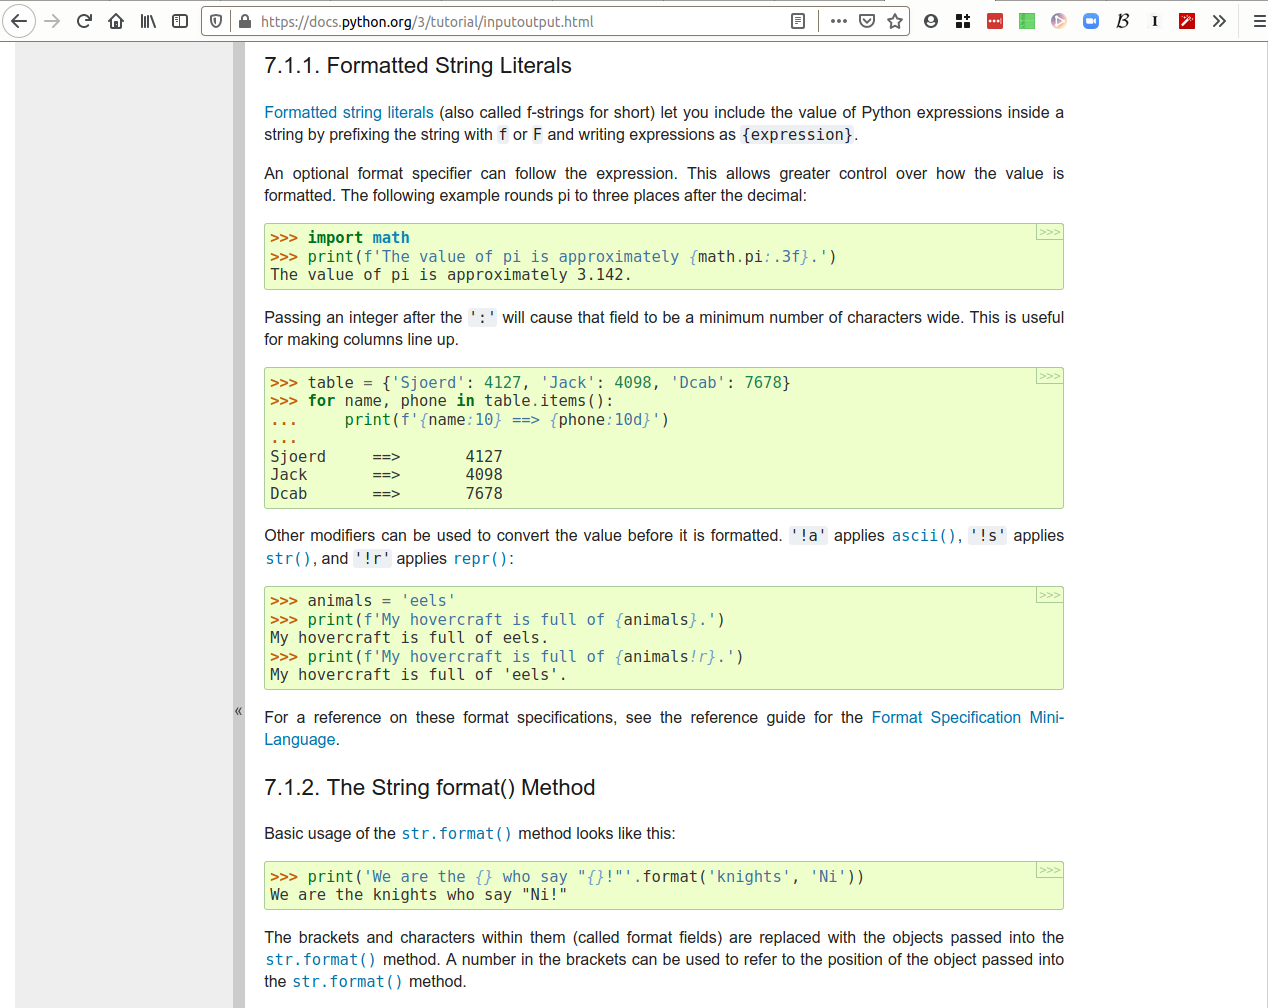
\includegraphics[width=\columnwidth]{figs/docs-strings.png}
\end{frame}


\subsection{Några fler saker man kan göra}

\begin{frame}
  \begin{example}[formatpi.py]
    \lstinputlisting{examples-more/formatpi.py}
  \end{example}
\end{frame}

\begin{frame}
  \begin{example}[align.py]
    \lstinputlisting{examples-more/align.py}
  \end{example}
\end{frame}

\begin{frame}
  \begin{example}[align-binary.py]
    \lstinputlisting{examples-more/align-binary.py}
  \end{example}
\end{frame}


\mode*
\mode<all>
\mode*

\section{Fel och felhantering}

\subsection{Särfall}

\begin{frame}[fragile]
  \begin{example}
    \begin{lstlisting}
>>> int("a")
Traceback (most recent call last):
  File "<stdin>", line 1, in <module>
ValueError: invalid literal for int() with base 10: 'a'
>>> 
    \end{lstlisting}
  \end{example}
\end{frame}

\begin{frame}[fragile]
  \begin{example}
    \begin{lstlisting}
>>> 5/0
Traceback (most recent call last):
  File "<stdin>", line 1, in <module>
ZeroDivisionError: division by zero
>>> 
    \end{lstlisting}
  \end{example}
\end{frame}

\begin{frame}[fragile]
  \begin{example}
    \begin{lstlisting}
>>> prynt(3)
Traceback (most recent call last):
  File "<stdin>", line 1, in <module>
NameError: name 'prynt' is not defined
>>> 
    \end{lstlisting}
  \end{example}
\end{frame}

\subsection{Felhantering: att fånga särfall}

\begin{frame}
  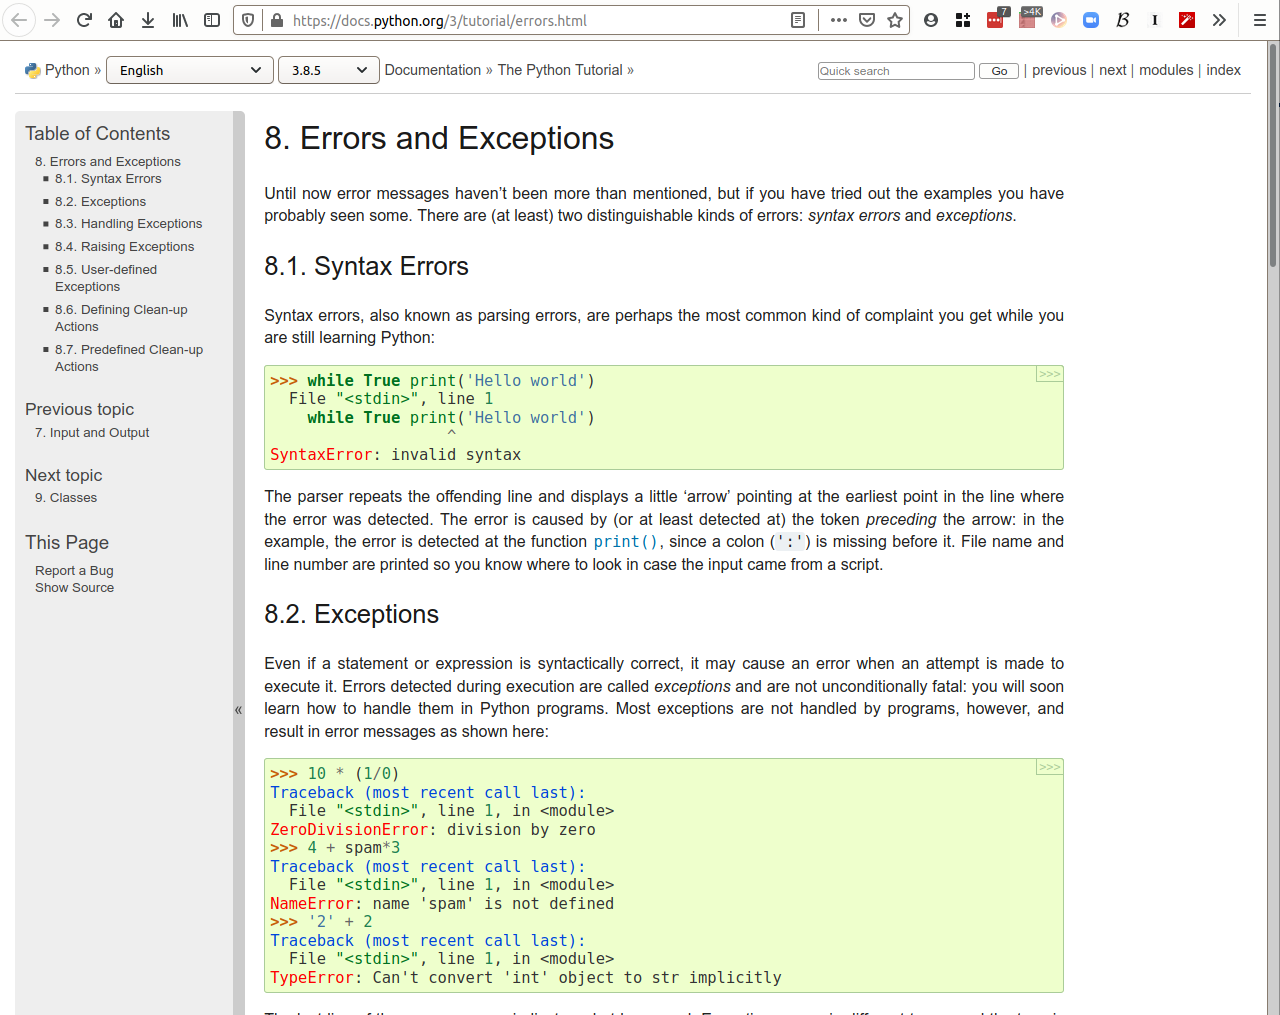
\includegraphics[width=\columnwidth]{figs/docs-except.png}
\end{frame}

\begin{frame}[fragile]
  \begin{example}[Fånga särfall: valuerr.py]
    \lstinputlisting{examples-more/valuerr.py}
  \end{example}

  \pause

  \begin{example}
    \begin{lstlisting}[language={}]
$ python3 valuerr.py
We caught this: invalid literal for int() with base 10: 'a'
    \end{lstlisting}
  \end{example}
\end{frame}

\begin{frame}[fragile]
  \begin{lstlisting}
try:
  # error
except Exception as err:
  print("Catch all errors!")
  \end{lstlisting}
  \begin{remark}
    \begin{itemize}
    \item \lstinline{except Exception as err} fångar \emph{allt}!
  \end{itemize}
  \end{remark}
\end{frame}

\begin{frame}[fragile]
  \begin{example}[manyerr.py]
    \lstinputlisting{examples-more/manyerr.py}
  \end{example}
\end{frame}


\mode*

\begin{frame}[allowframebreaks]
  \printbibliography
\end{frame}
\end{document}
